\documentclass{article}
\usepackage[utf8]{inputenc}

\usepackage[utf8]{inputenc}
\usepackage[spanish,es-tabla,es-nodecimaldot]{babel}
\usepackage{amsmath,amsthm,amsfonts,amssymb,mathtools,dsfont,mathrsfs}
\usepackage{enumerate,graphicx,xcolor}
\usepackage{lmodern}
\usepackage[T1]{fontenc}
\usepackage[left=2cm,top=2.5cm,right=2cm,bottom=2.5cm]{geometry}
\usepackage[activate={true,nocompatibility},final,tracking=true,kerning=true,spacing=true,factor=1100,stretch=10,shrink=10]{microtype}
\usepackage{hyperref}


%\DeclarePairedDelimiter{\norm}{\lVert}{\rVert}




\newcommand{\N}{\mathbb{N}}
\newcommand{\R}{\mathbb R}
\newcommand{\Z}{\mathbb Z}
\newcommand{\Rbar}{\overline{\mathbb R}}
\newcommand{\F}{\mathscr F}
\newcommand{\A}{\mathscr A}
\newcommand{\To}{\Rightarrow}
\newcommand{\C}{\mathscr C}
\newcommand{\La}{\mathscr L_A}
\newcommand{\B}{\mathcal B}
\newcommand{\Q}{\mathbb Q}
\renewcommand{\epsilon}{\varepsilon}
\renewcommand{\L}{\mathcal L}
\renewcommand{\d}{\mathrm d}
\newcommand{\abs}[1]{\left| #1 \right|}
\newcommand{\pts}[1]{\left( #1 \right)}
\newcommand{\norm}[1]{\left\lVert#1\right\rVert}
\renewcommand{\P}[1]{\mathbb P\left( #1 \right)}
\newcommand{\E}[1]{\mathbb E \left( #1 \right)}


\newcommand{\ols}[1]{\mskip.5\thinmuskip\overline{\mskip-.5\thinmuskip {#1} \mskip-.5\thinmuskip}\mskip.5\thinmuskip} % overline short
\newcommand{\olsi}[1]{\,\overline{\!{#1}}} % overline short italic
\makeatletter
\newcommand\closure[1]{
  \tctestifnum{\count@stringtoks{#1}>1} %checks if number of chars in arg > 1 (including '\')
  {\ols{#1}} %if arg is longer than just one char, e.g. \mathbb{Q}, \mathbb{F},...
  {\olsi{#1}} %if arg is just one char, e.g. K, L,...
}
% FROM TOKCYCLE:
\long\def\count@stringtoks#1{\tc@earg\count@toks{\string#1}}
\long\def\count@toks#1{\the\numexpr-1\count@@toks#1.\tc@endcnt}
\long\def\count@@toks#1#2\tc@endcnt{+1\tc@ifempty{#2}{\relax}{\count@@toks#2\tc@endcnt}}
\def\tc@ifempty#1{\tc@testxifx{\expandafter\relax\detokenize{#1}\relax}}
\long\def\tc@earg#1#2{\expandafter#1\expandafter{#2}}
\long\def\tctestifnum#1{\tctestifcon{\ifnum#1\relax}}
\long\def\tctestifcon#1{#1\expandafter\tc@exfirst\else\expandafter\tc@exsecond\fi}
\long\def\tc@testxifx{\tc@earg\tctestifx}
\long\def\tctestifx#1{\tctestifcon{\ifx#1}}
\long\def\tc@exfirst#1#2{#1}
\long\def\tc@exsecond#1#2{#2}
\makeatother

\newtheorem{lemma}{Lema}
\newtheorem{theorem}{Teorema}

\setlength\parindent{0pt}
\setlength\parskip{4pt}


\title{Cómputo científico para probabilidad y estadística. Tarea 2.\\
Descomposición QR y mínimos cuadrados.}
\author{Juan Esaul González Rangel}
\date{Septiembre 2023}



\begin{document}

\maketitle


\begin{enumerate}

    \item Implementar el algoritmo de Gram-Schmidt modificado 8.1 del Trefethen (p. 58) para generar 
    la descomposición $QR$.

    En el archivo \texttt{QR.py}, el algoritmo está implementado en la función \texttt{QR}. 

    \item Implementar el algoritmo que calcula el estimador de mínimos cuadrados
    en una regresión usando la descomposición $QR$.

    En el archivo \texttt{QR.py}, el algoritmo está implementado en la función \texttt{LSQR}. 

    \item Generar $\mathbf Y$ compuesto de $y_i = \sen(x_i) + \epsilon_i$ donde 
    $\epsilon_i \sim N (0, \sigma)$ con $\sigma = 0.11$ para $x_i = \frac{4\pi i}n$ para 
    $i = 1, \dots , n$.

    Hacer un ajuste de mínimos cuadrados a $\mathbf Y$, con descomposición $QR$, ajustando un polinomio 
    de grado $p - 1$.

    \begin{itemize}
        \item Considerar los 12 casos: $p = 3, 4, 6, 100$ y $n = 100, 1000, 10000$.
        
        En el archivo \texttt{.py} está implementada la regresión polinómica para los valores
        dados.

        \item Graficar el ajuste en cada caso.
        
        Las siguientes gráficass muestran el ajuste obtenido en cada caso.

       \begin{center}
            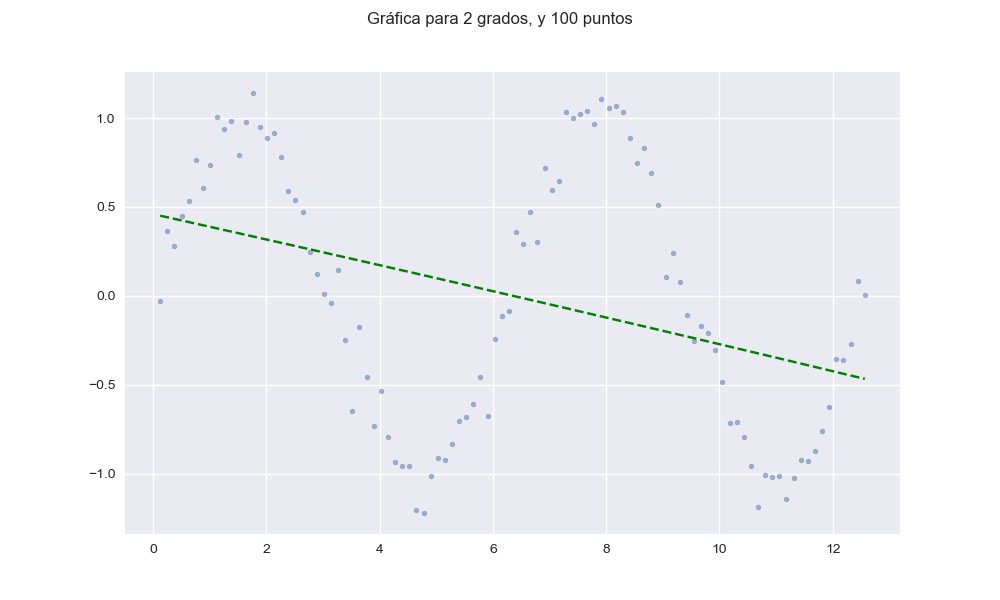
\includegraphics[width=\textwidth]{Ajuste2100.png}
       
            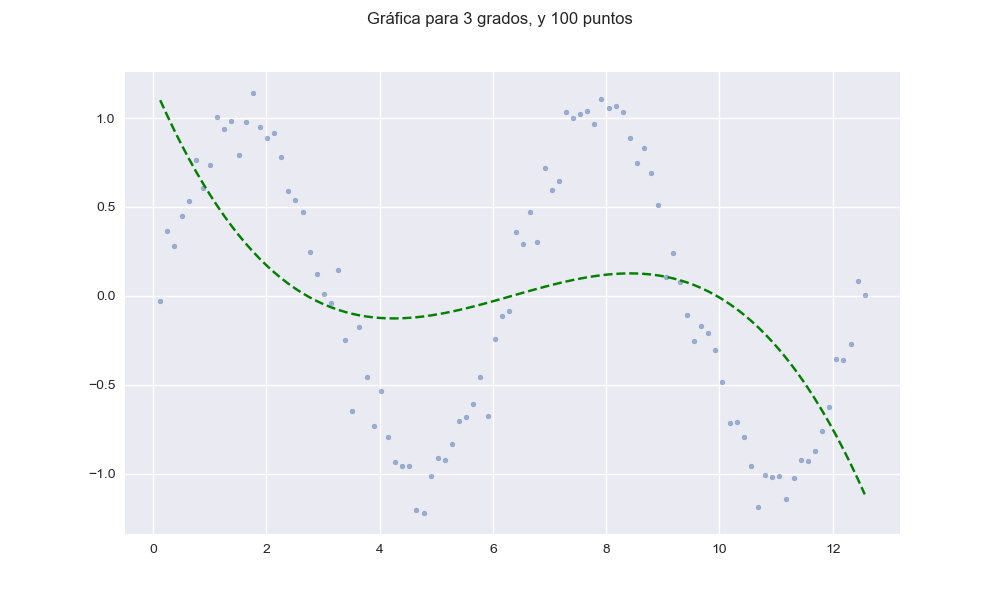
\includegraphics[width=\textwidth]{Ajuste3100.png}
       
            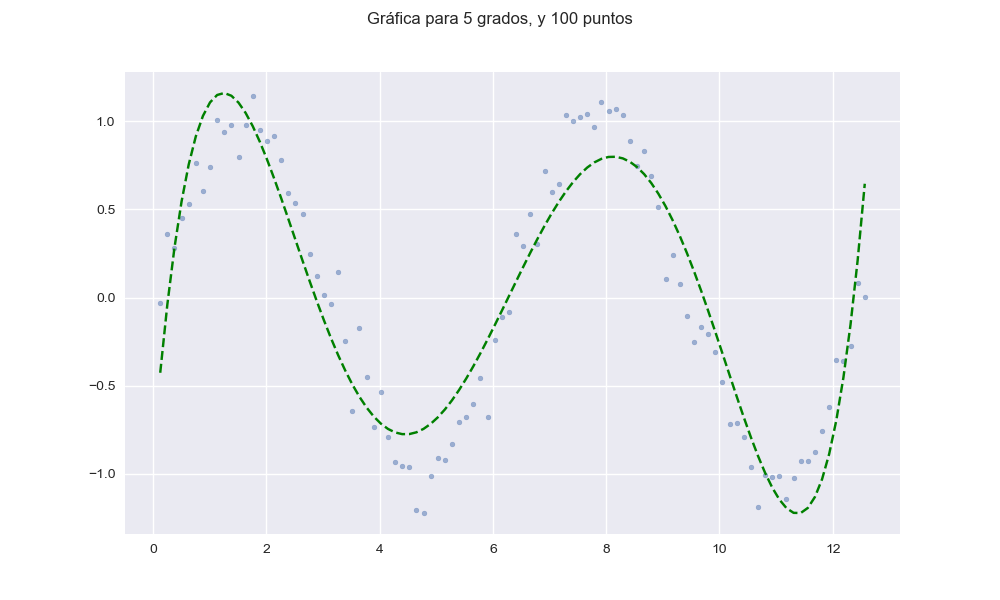
\includegraphics[width=\textwidth]{Ajuste5100.png}
        
            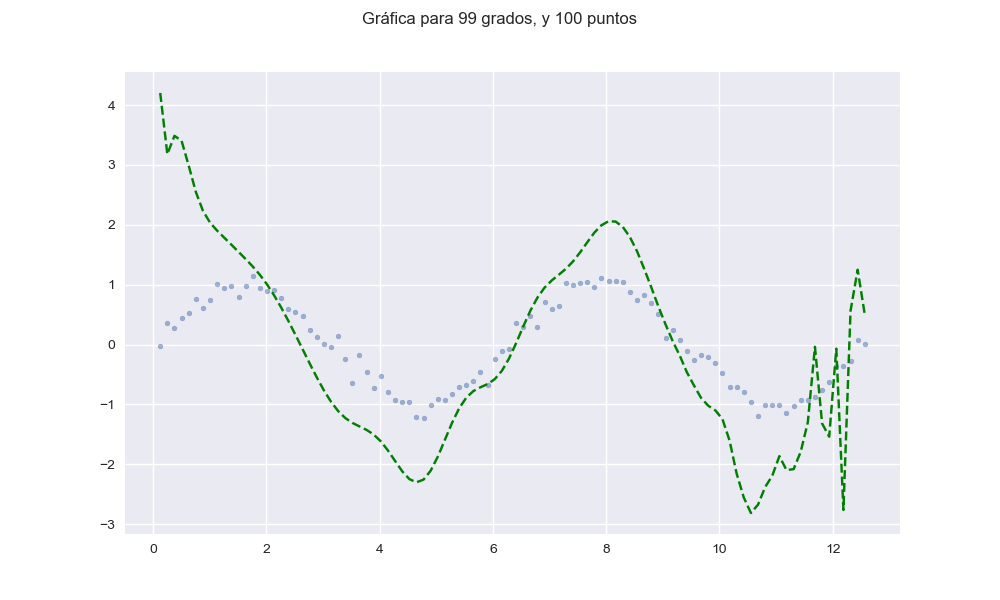
\includegraphics[width=\textwidth]{Ajuste99100.png}
      
            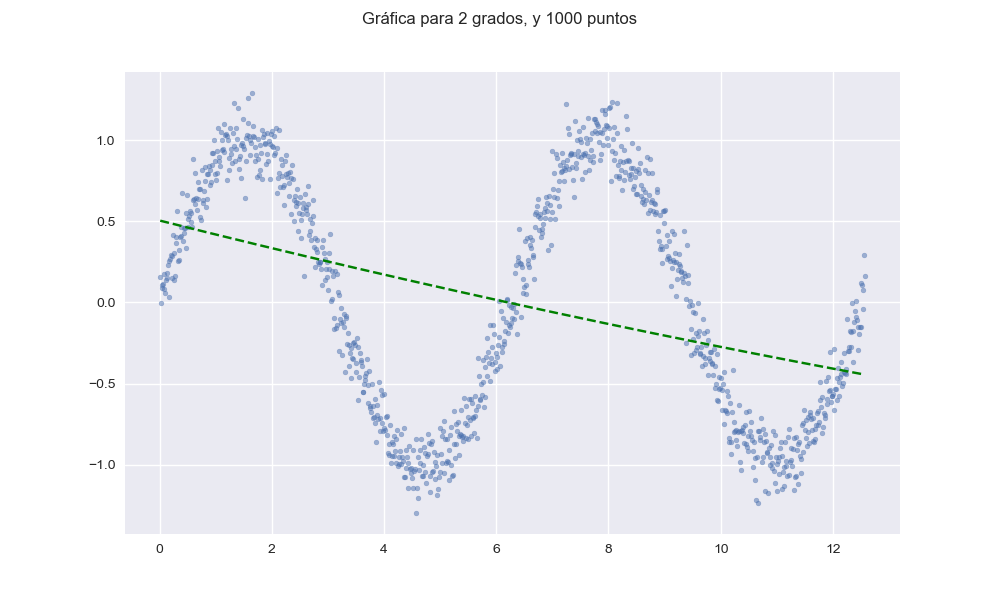
\includegraphics[width=\textwidth]{Ajuste21000.png}
        
            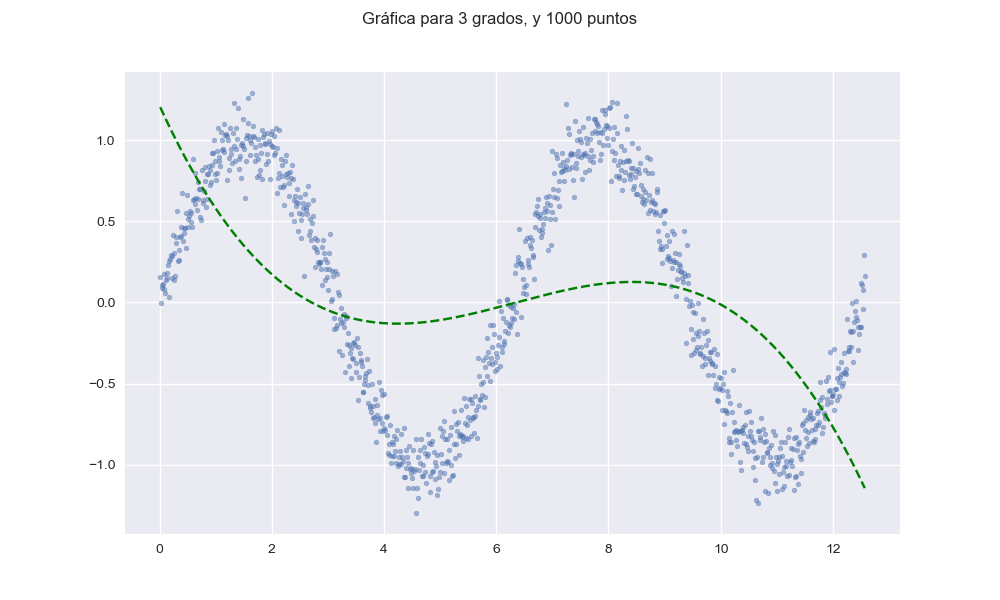
\includegraphics[width=\textwidth]{Ajuste31000.png}
       
            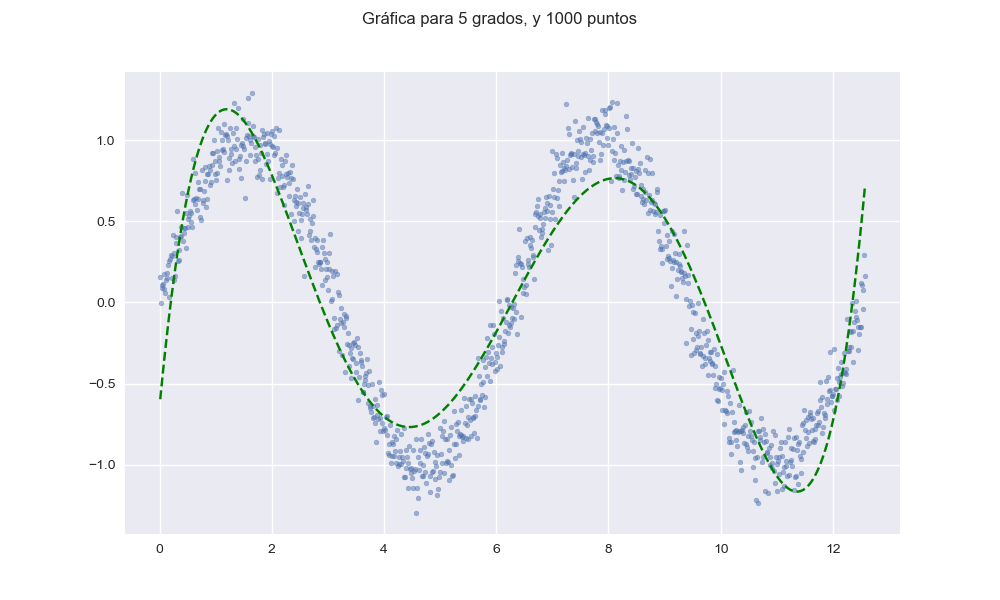
\includegraphics[width=\textwidth]{Ajuste51000.png}
        
            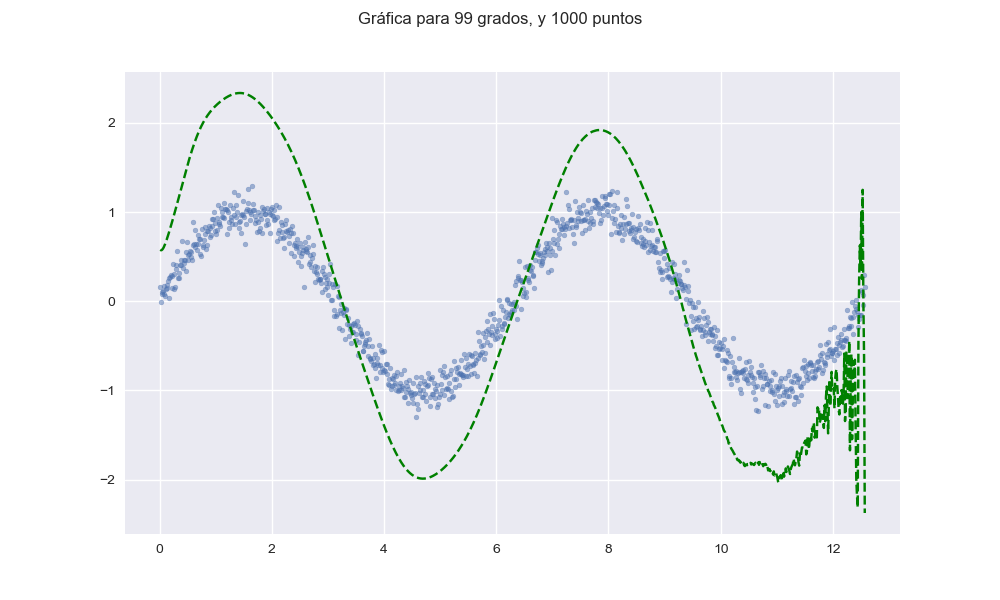
\includegraphics[width=\textwidth]{Ajuste991000.png}
        
            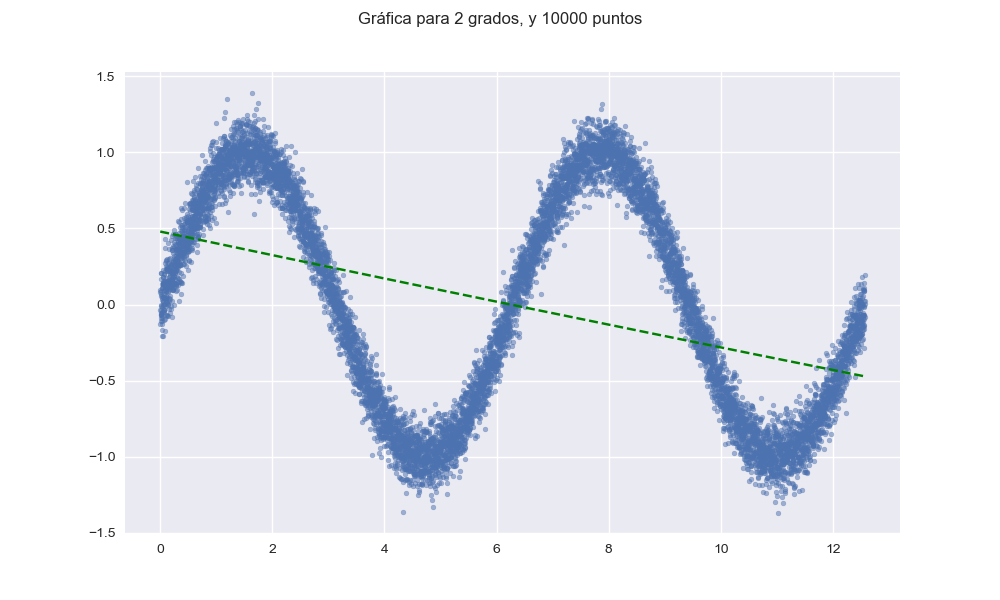
\includegraphics[width=\textwidth]{Ajuste210000.png}
        
            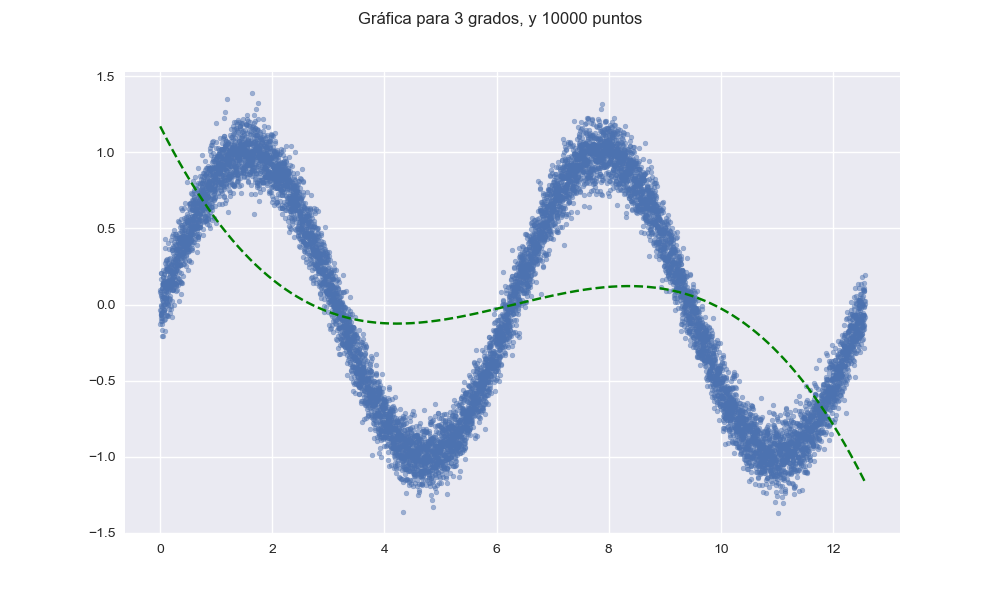
\includegraphics[width=\textwidth]{Ajuste310000.png}
        
            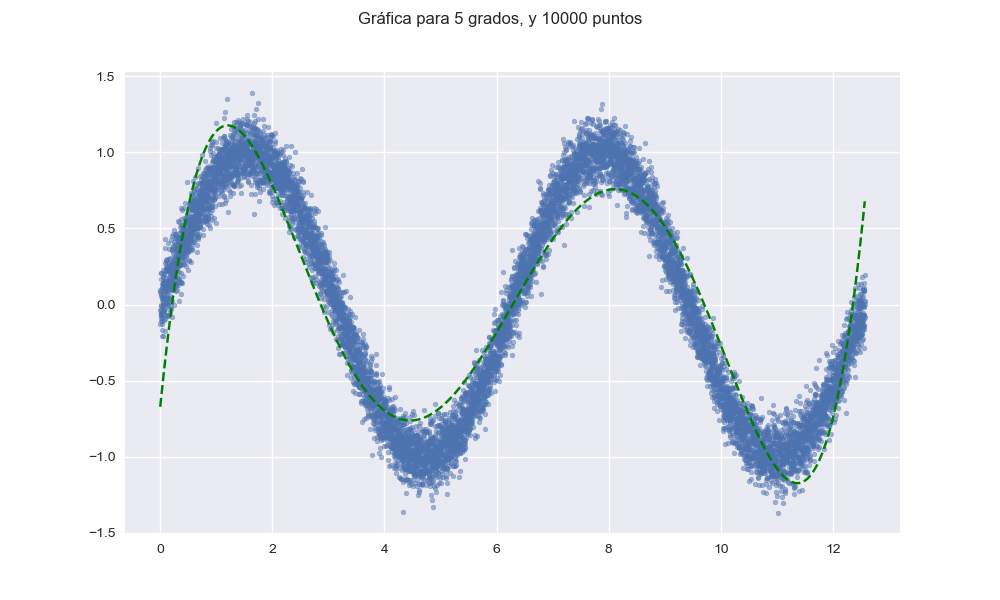
\includegraphics[width=\textwidth]{Ajuste510000.png}
        
            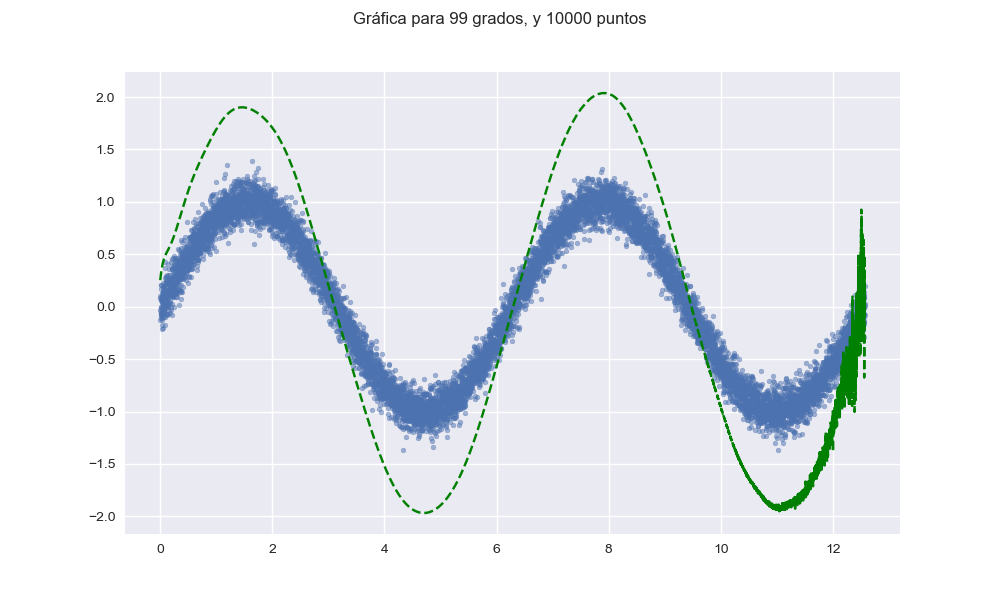
\includegraphics[width=\textwidth]{Ajuste9910000.png}
        \end{center}

        Como podemos observar, el mejor ajuste para cualquier cantidad de puntos
        se logra cuando se utiliza un polinomio de grado 5, para grados menores, la 
        curva ajustada resulta muy insuficiiente, y para grados mayores, tiende a presentar
        demasiadas oscilaciones, lo que indica un comportamiento irregular que está 
        más influido por el ruido.

        Cabe resaltar también que cuando aumenta el grado del polinomio de manera 
        considerable, la precisión del ajuste decrece al punto de que los límites de la función
        se mueven de $(-1,1)$ a $(-2,2)$. Esto puede tener su causa en que con una cantidad de
        columnas tan grande, el número de cndición de la matriz crece considerablemente, llegando
        a ser en uno de los casos del orden de $10^{111}$, sin embargo, cuando aumenta el número de
        filas manteniendo el número de columnas relativamente pequeño, el número de condición parece
        crecer más lentamente, teniendo para una matriz $(10000\times 6)$ un número de condición del
        orden de $100^6$.

        

        \item Medir tiempo de ejecución de su algoritmo, comparar con descomposición $QR$ de 
        \texttt{scipy} y graficar los resultados.

        En la siguiente figura tenemos una comparación entre los tiempos de ejecución del algoritmo
        propio y el algoritmo de \texttt{scipy} para la descomposición QR. Podemos notar que para
        vaalores pequeños de $p-1$, ambos algoritmos tienen tiempos de ejecución bastante similares,
        incluso cuando $n$ es muy grande, sin embargo, a medida que crece $p$, se nota una diferencia
        sustancial, incluso manteniendo el valor $n$ pequeño. 

        \begin{center}
            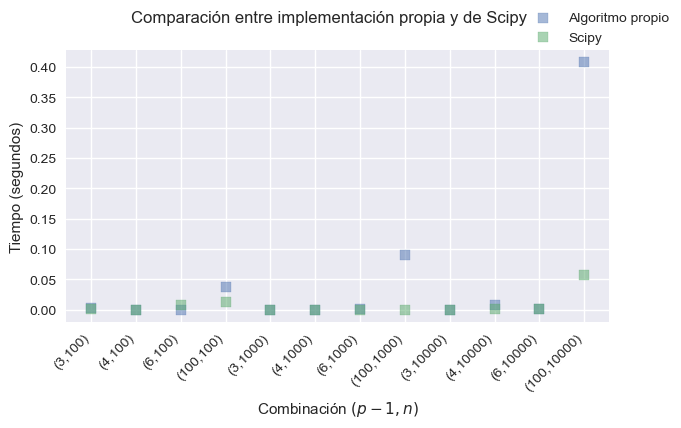
\includegraphics[width=0.8\textwidth]{qr-compar.png}
        \end{center}

    \end{itemize}


    \item Hacer $p = 0.1n$, o sea, diez veces más observaciones que coeficientes en la regresión, 
    ¿Cual es la $n$ máxima que puede manejar su computadora?

    Con un bloque \texttt{try}-\texttt{except} de \texttt{Python} corrimos el algoritmo para los 
    tamaños $50, 75, 100, 125, 150, 155, 281$ y $300$ para $p$ (definiendo $n=10*p$) después de varias pruebas. Aunque en varios casos
    el algoritmo logra terminar su ejecución, esto no significa que todos los resultados que se obtienen
    sean útiles. En particular, se encontraron las siguientes observaciones:

    \begin{itemize}
        \item Para valores de $n$ menores a $1550$, el algoritmo se ejecuta con normalidad y todas las entradas
        del vector de coeficientes son no nulas, lo que parece indicar que aún es información útil.
        \item Cuando pasamos a $n=1560$, las últimas entradas del vector comienzan a ser idénticas a 0, independientemente
        de los puntos ajustados, lo que indica que posiblemente comienza a haber valores fuera del rango de precisión de
        punto flotante que maneja la máquina, este patrón continúa, agregando cada vez más ceros en la parte final
        del vector de coeficientes, hasta el punto en que prácticamente todos son iguales a cero.
        \item A partir de $n=2800$ encontraos varios avisos con \texttt{Runtime error}, lo que indica que existen
        problemas con la aritmética del punto flotante que estamos usando, ya sea valores que escapan del rango del
        sistema de punto flotante, u operaciones inválidas. Esto confirma que coeficientes obtenidos con este tamaño
        de matriz no son realmente útiles en la práctica (al menos con esta implementación).
        \item Cuando usamos matrices con $n$ aproximadamente igual a $3000$ obtenemos que varios de los valores
        se vuelven un \texttt{nan}, es decir, un objeto que resulta de una operación en la que no fue posible 
        obtener un valor numérico como resultado, la falla de nuevo es que hay operaciones que escapan de la precisión
        del sistema de punto flotante. Evidentemente, estos valores no son útiles para su implementación en ningún contexto.
    \end{itemize}

    En resumen, aunque la computadora puede correr el programa para tamaños de matriz muy grande, hay que tener en
    cuenta que la precisión de las operaciones se va perdiendo cada vez que incrementamos el tamaño de la matriz (y 
    por lo tanto su número de condición), lo que causa, que aunque tengamos valores como salida de la ejecucion, no es
    recomendable utilizarlos. Según lo observado en los experimentos anteriores, el tamaño más grande que es seguro 
    para su uso en el caso en que $n = 10p$ es $1550\times155$.
    % Hasta $1560 \times 156$ obtenemos resultados no nulos. En $2800 \times 280$ obtenemos 
    % \texttt{Runtime error} y en $3000\times 300$ obtenemos \texttt{nan} como resultado.
   
\end{enumerate}




 \end{document}